% !TEX TS-program = xelatex
% !TEX encoding = UTF-8

%%%%%%%%%%%%%%%%%%%%%%%%%%%%%%%%%%%%%%%%%%%%%%%%%%%%%%%%%%%%%%%%%
%% Resume template - https://github.com/lquesada/resume
%% Check that URL for licensing information.
%% 
%% Copyright (c) 2024, Luis Quesada -
%% https://github.com/lquesada | www.luisquesada.com
%%
%% Heavily based of (an old version of) the SIMPLE-RESUME-CV
%% by zachscrivena.
%% <https://github.com/zachscrivena/simple-resume-cv>
%%%%%%%%%%%%%%%%%%%%%%%%%%%%%%%%%%%%%%%%%%%%%%%%%%%%%%%%%%%%%%%%%

%%%%%%%%%%%%%%%%%%%%%%%%%%%%%%%%%%%%%%%%%%%%%%%%%%%%%%%%%%%%%%%%%
%% INSTRUCTIONS FOR COMPILING THIS DOCUMENT ("resume.tex")
%% TEX ---(XeLaTeX)---> PDF:
%%
%% Method 1: Use latexmk for fully automated document generation:
%%   latexmk -xelatex "resume.tex"
%%   (add the -pvc switch to automatically recompile on changes)
%%
%% Method 2: Use XeLaTeX directly:
%%   xelatex "resume.tex"
%%   (run multiple times to resolve cross-references if needed)
%%
%% PDF ---(pdf2htmlEX)> HTML:
%%
%% Install pdf2htmlEX from https://github.com/coolwanglu/pdf2htmlEX, then:
%%   alias pdf2htmlEX='docker run -ti --rm -v `pwd`:/pdf bwits/pdf2htmlex pdf2htmlEX'
%%   pdf2htmlEX --zoom 1.5 --process-outline 0 resume.pdf
%%
%%%%%%%%%%%%%%%%%%%%%%%%%%%%%%%%%%%%%%%%%%%%%%%%%%%%%%%%%%%%%%%%%

% Note: Search "SIZEMARKER" to find settings you can tweak to
%       make the page, the margins, or the text bigger or smaller.


% SIZEMARKER: You may want to replace "letterpaper" with "a4paper", but when
% exporting to html, letterpaper can be printed in both letter and A4 sheets
% of paper.
% SIZEMARKER: You may also want to tweak the font size.
\documentclass[letterpaper,10pt,oneside]{article}

% Long table for page layout.
\usepackage{longtable}
\usepackage{calc}

% SIZEMARKER: Page margins
\usepackage[
left=0.37in,
right=0.65in,
top=0.85in,
bottom=0.45in,
nohead,
includefoot]{geometry}

% Hyphenation: Disabled.
\usepackage[none]{hyphenat}

% XeLaTeX packages.
\usepackage{fontspec}
\defaultfontfeatures{Ligatures=NoTeX}
\usepackage{xunicode}
\usepackage{xltxtra}
\usepackage{xcolor}
\usepackage[export]{adjustbox}

\renewcommand*{\familydefault}{\sfdefault}


% PDF settings and properties.

% Headers and footers: Blank header, page number in footer.
% Commented: I don't want the page number in footer.
\makeatletter
\def\ps@plain{%
\def\@oddhead{}%
\def\@evenhead{}%
\def\@oddfoot{}%
\def\@evenfoot{}}
%\def\@oddfoot{\footnotesize\hfill{Page}~{\thepage}~of~\pageref{LastPage}\hfill}%
%\def\@evenfoot{\footnotesize\hfill{Page}~{\thepage}~of~\pageref{LastPage}\hfill}}
\makeatother

\pagestyle{plain}

% Paragraph style: No indentation.
\setlength{\parindent}{0in}

% SIZEMARKER: Line spacing
\renewcommand{\baselinestretch}{1.23}

\newcommand{\DatestampY}[1]{#1}

% SIZEMARKER: Item spacing
\newcommand{\itemspacing}{\vspace{0.10cm}}

% SIZEMARKER: Item spacing for second page
\newcommand{\itemspacingtwo}{\vspace{0.04cm}}
\newcommand{\portfoliospacing}{\vspace{1.0cm}}

% Hidden link
\definecolor{hiddenblue}{HTML}{600030}
\newcommand{\sref}[2]{%
    \href{https://0/local/attachments/#1}{\textcolor{blue}{#2}}% % Replace with color hiddenblue if I want them hidden again
}


% Macro: body (rest of the document).
% SIZEMARKER: Left vs. right columns
\newenvironment{body}
{\par\par
\begin{longtable}{p{0.145\textwidth}p{0.81\textwidth}}}
{\par\end{longtable}\par}

\newenvironment{portfoliobody}
{\par\par
\begin{longtable}{p{0.22\textwidth}p{0.735\textwidth}}}
{\par\end{longtable}\par}

% Macro: section (new section for Education, Research Experience, etc.).
% SIZEMARKER: The separation here is between sections.
\renewcommand{\section}[3]{\\[-0.40cm]\pdfbookmark[2]{#2}{#3}\\%
\raggedleft  %align to the right
{\fontsize{9.5pt}{9.5pt}\selectfont\bfseries\raggedright%
\MakeUppercase{#1}}&}

% SIZEMARKER: SmallEntryGap is a small vertical gap within a long entry
\newcommand{\SmallEntryGap}{\par\vspace{0.38em}\par} 

% Round image
\usepackage{tikz}

\newcommand{\roundpic}[4][]{
\tikz\node [circle, minimum width = #2,
path picture = {
\node [#1] at (path picture bounding box.center) {
\includegraphics[width=#3]{#4}};
}] {};}


%%%%%%%%%%%%%%%%%%%%%%%%%%%%%%%%%%%%%%%%%%%%%%%%%%%%%%%%%%%%%%%%%
%% PREAMBLE.
%%%%%%%%%%%%%%%%%%%%%%%%%%%%%%%%%%%%%%%%%%%%%%%%%%%%%%%%%%%%%%%%%


% CV Info (to be customized).
\newcommand{\CVTitle}{Luis Quesada - Resume}
\newcommand{\CVNote}{CV compiled on {\today}}

% PDF settings and properties.
\usepackage{hyperref}
\hypersetup{
pdftitle={\CVTitle},
pdfauthor={Luis Quesada},
pdfcreator={},
pdfproducer={},
pdfkeywords={},
pdfpagemode={},
bookmarks=true,
unicode=true,
bookmarksopen=true,
pdfstartview=FitH,
pdfpagelayout=OneColumn,
pdfpagemode=UseOutlines,
hidelinks,
breaklinks,
colorlinks=true,
linkcolor=blue,
citecolor=blue,
filecolor=blue,
urlcolor=blue
}

%%%%%%%%%%%%%%%%%%%%%%%%%%%%%%%%%%%%%%%%%%%%%%%%%%%%%%%%%%%%%%%%%
%% ACTUAL DOCUMENT.
%%%%%%%%%%%%%%%%%%%%%%%%%%%%%%%%%%%%%%%%%%%%%%%%%%%%%%%%%%%%%%%%%

\begin{document}


%%%%%%%%%%%%%%%
% TITLE BLOCK %
%%%%%%%%%%%%%%%

\begin{center}\begin{longtable}{p{0.245\textwidth}p{0.62\textwidth}}
\raggedleft\roundpic{3.2cm}{3.2cm}{pic.jpg}\hspace{0.3cm} % SIZEMARKER
&
\vspace{-2.93cm} \par
\huge{\textbf{Luis Quesada}} \par
\large{\textbf{Senior Software Engineering Manager}} \par
\normalsize{\href{https://lquesada.github.io/resume/}{www.luisquesada.com} | \href{http://github.com/lquesada}{github.com/lquesada}}\par
\normalsize{Contact via \href{https://www.linkedin.com/in/luisquesadatorres}{linkedin.com/in/luisquesadatorres}}\par
\normalsize{See recommendations \href{https://www.linkedin.com/in/luisquesadatorres/details/recommendations/}{here}}

\end{longtable}\end{center}

\vspace{-2.05cm} % SIZEMARKER

\newenvironment{comp}
{
\vspace{-0.55\baselineskip} % SIZEMARKER
\begin{itemize}
\setlength{\itemsep}{0pt}
\setlength{\parskip}{0pt}
\setlength{\parsep}{0pt}
\setlength{\partopsep}{0pt}
\setlength{\topsep}{0pt}
}
{
\end{itemize}
\vspace{-0.5\baselineskip} % SIZEMARKER
}



\begin{body}

%%%%%%%%%%%%%%%
%%  SUMMARY  %%
%%%%%%%%%%%%%%%

\section{Summary}{Summary}{PDF:Summary}

Engineering leader with expertise in defining and executing technical strategy, with a proven track record of building top-performing organizations. Led 70+ engineers to revamp five production areas across 50+ products, boosting engineering velocity and system reliability and efficiency for 1K+ engineers.

%%%%%%%%%%%%%%%
%%  SKILLS   %% Summarized as languages section
%%%%%%%%%%%%%%%

%\section{Skills}{Skills}{PDF:Skills}
%Generative Artificial Intelligence: Infrastructure, solutions, and application of multi-modal models\newline
%Systems: Architecture, performance, automation, monitoring, load balancing, capacity, and data integrity\newline
%Computer Languages: Go, Java, Python, JavaScript, TypeScript, PHP, Bash shell script, and SQL\newline
%People: Organization design, career development, team health, coaching, presentation, and negotiation\newline
%Languages: Spanish (Native), English (\sref{Diploma-ESOLCPE.pdf}{C2}), German (\sref{Diploma-GoetheDeutsch-B2.pdf}{B2}), Swiss German (B1), and Esperanto (\sref{Diploma-EAB-Esperanto-Meznivela.pdf}{B1})

%%%%%%%%%%%%%%%%
%% INDUSTRY %%
%%%%%%%%%%%%%%%%

\section{Industry}{Industry}{PDF:Industry}

\textbf{Google}, \DatestampY{2014} -- currently \vspace{0.06cm} \newline
\phantom{g}\textbf{Geo, Software Engineering} \textemdash{ }Senior Engineering Manager (L7)
\begin{comp}
\item Developing Google-wide infrastructure, both applying and serving generative artificial intelligence
\end{comp}
\itemspacing

\phantom{g}\textbf{YouTube Trust \& Safety, Software Engineering} \textemdash{ }Senior Engineering Manager (L7)
\begin{comp}
\item Improved the performance of high-throughput pipelines by \textbf{1000x}. \textbf{Award}: \sref{Google-Award-PerformanceExcellence.pdf}{Performance Excellence}
\item Developed Large Language Model infrastructure and tooling, used by \textbf{40+} engineering projects and \textbf{300+} analysts to define complex insights. \textbf{Awards}: \sref{Award-EngineeringExcellenceImpact.pdf}{Engineering} + \sref{Google-Award-FeatureExcellence.pdf}{Feature} + \sref{Google-Award-FeatureExcellence2.pdf}{Feature} Excellence
\end{comp}
\itemspacing

\phantom{g}\textbf{Cloud Artificial Intelligence, Site Reliability Engineering} \textemdash{ }Senior Engineering Manager (L5$\rightarrow$L7)
\begin{comp}
\item Led the productionization of three flagship products. Unblocked \textbf{\$1B+} revenue.
\item Redesigned capacity management, monitoring, rollouts, data integrity, and frameworks across \textbf{1K+} engineers. Saved \textbf{\$XXXM+} in computing resources and improved the reliability of \textbf{50+} products. \textbf{Awards}: \sref{Google-Award-GoogleCloudTechImpact-2022.pdf}{Cloud} + \sref{Google-Award-CoreTechImpact-2021.pdf}{Core} + \sref{Google-Award-GoogleTechImpact-2022.pdf}{Google Tech} Impact, \sref{Google-Award-Perfy.pdf}{Perfy}, \sref{Google-Award-TechDebtBusters1.pdf}{Tech Debt Busters}, \sref{Google-Award-TechDebtBusters2.pdf}{Tech Debt Busters}
\end{comp}
\itemspacing

\phantom{g}\textbf{Datacenter Software, Site Reliability Engineering} \textemdash{ }Technical Leader/Engineering Manager (L5)
\begin{comp}
\item Led the revamp of critical datacenter systems. Sped up the launch by one year.
\end{comp}
\itemspacing

\phantom{g}\textbf{Apps Storage, Site Reliability Engineering} \textemdash{ }Senior Software Engineer, Technical Leader (L4$\rightarrow$L5)
\begin{comp}
\item Deployed capacity models for products with \textbf{1B+} users. Saved \textbf{\$XXXM+} in computing resources.
\item Led the company-wide migration to a new storage service. \textbf{Award}: \sref{Google-Award-FeatsOfEngineering-2018.pdf}{Feats of Engineering}
\end{comp}
\itemspacing

%%%%%%%%%%%%%%%
%% ADVOCACY %%
%%%%%%%%%%%%%%%
\section{Advocacy}{Advocacy}{PDF:Advocacy}
\textbf{People Leadership}
\begin{comp}
\item Co-authored a chapter on \href{https://landing.google.com/sre/workbook/chapters/overload/}{team overload} for \textit{The Site Reliability Workbook} published by \textbf{O'Reilly}.
\item Designed and scaled the \textit{Leadership Wheel of Misfortune} program to hundreds of sessions globally.
\item Mentored and coached hundreds of engineers, technical leaders, managers, interns, and apprentices.
\item Keynote speaker on career and technical topics at various universities.
\end{comp}

\textbf{Technical Influence}
\begin{comp}
\item Published an article on \href{https://static.googleusercontent.com/media/sre.google/en//static/pdf/login\_winter20\_10\_torres.pdf}{best practices for capacity management}.
\item Published talks on \href{https://youtu.be/dhTVVWzpc4Q}{Google production environment}, \href{https://youtu.be/pOo0oKNM9I8}{resources}, and \href{https://youtu.be/d7nAGI\_NZPk}{Paxos}. Achieved \textbf{210K views}.
\end{comp}

%%%%%%%%%%%%%%%
%% EDUCATION %%
%%%%%%%%%%%%%%%
\section{Education}{Education}{PDF:Education}
\textbf{University of Granada}, \DatestampY{2004} -- \DatestampY{2014} \newline
\phantom{g}Research fellow on \href{https://doi.org/10.1142/S0129065712500190}{computer vision} and \href{https://doi.org/10.1142/S0218194014500375}{compilers}, led a thesis on \href{https://github.com/lquesada/ADAgio}{music languages}. \textbf{Award}: \sref{UGR-Award-BestMasterThesis-MusicPrototyping.pdf}{Best Thesis}.
\phantom{g}\textit{\sref{MRes-SoftComputingArtificialIntelligence-Diploma.pdf}{Master in Research}, Soft Computing and Intelligent Systems}. GPA \sref{MRes-SoftComputingArtificialIntelligence-Transcript-Spanish.pdf}{9.3/10}.\newline
\phantom{g}\textit{\sref{BSc-ManagementInformationTechnology-Diploma.pdf}{Bachelor of Science}, \sref{BSc-ManagementInformationTechnology-Transcript.pdf}{Information Systems Engineering}}. GPA \sref{BSc-ManagementInformationTechnology-Transcript-Spanish.pdf}{8.7/10}. \textbf{Award}: \sref{BSc-ManagementInformationTechnology-Award-FirstOfPromotion.pdf}{1st in Class}.\newline
\phantom{g}\textit{\sref{MSc-ComputerEngineering-Diploma.pdf}{Master of Science}, \sref{MSc-ComputerEngineering-Transcript.pdf}{Computer Science}}. GPA \sref{MSc-ComputerEngineering-Transcript-Spanish.pdf}{9.2/10}. \textbf{Awards}: \sref{MSc-ComputerEngineering-Award-FirstOfPromotion.pdf}{1st in Class}, \sref{MSc-ComputerEngineering-Award-NationalAward.pdf}{National Award}, \sref{MSc-ComputerEngineering-Award-BestMasterThesis.pdf}{Best Thesis}.\newline
\phantom{g}\textit{\sref{BSc-SystemInformationTechnology-Diploma.pdf}{Bachelor of Science}, \sref{BSc-SystemInformationTechnology-Transcript.pdf}{Computer Systems Engineering}}. GPA \sref{BSc-SystemInformationTechnology-Transcript-Spanish.pdf}{8.7/10}. \textbf{Award}: \sref{BSc-SystemInformationTechnology-Award-FirstOfPromotion.pdf}{1st in Class}.

%%%%%%%%%%%%%%%%%%%
%%  CERTIFICATES %%
%%%%%%%%%%%%%%%%%%%
%\section{Certificates}{Certificates}{PDF:Certificates}
%\sref{Certificate-Coursera-IBM-GenerativeAIEngineering.pdf}{Professional Certificate on Generative Artificial Intelligence Engineering} \textemdash{ }IBM, \DatestampY{2024} \newline
%\sref{Certificate-Coursera-IBM-AIDeveloper.pdf}{Professional Certificate on Artificial Intelligence Development} \textemdash{ }IBM, \DatestampY{2024} \newline
%\sref{Certificate-Coursera-Google-Cybersecurity.pdf}{Professional Certificate on Cybersecurity} \textemdash{ }Google, \DatestampY{2024} \newline
%\sref{Certificate-Certyred.pdf}{Professional Certificate on Security} \textemdash{ }University of Salamanca, \DatestampY{2011} \newline
%\sref{Certificate-Coursera-Google-UX-Design.pdf}{Professional Certificate on User Experience Design} \textemdash{ }Google, \DatestampY{2024} \newline
%\sref{Certificate-HAREC.pdf}{Harmonized Amateur Radio Exam Certificate} \textemdash{ }Ofcom, \DatestampY{2025}
%\sref{Diploma-BerkleeCollege-ModernMusician.pdf}{Modern Musician Specialization} \textemdash{ }Berklee College of Music, \DatestampY{2014} \newline
%\sref{Diploma-ABRSM-MusicTheory5.pdf}{Grade 5 Music Theory} \textemdash{ }The Associated Board of the Royal Schools of Music, \DatestampY{2013} \newline
%\sref{Diploma-ABRSM-SingingGrade4.pdf}{Grade 4 Singing} \textemdash{ }The Associated Board of the Royal Schools of Music, \DatestampY{2013}

%%%%%%%%%%%%%%%
%% LANGUAGES %%
%%%%%%%%%%%%%%%

\section{Languages}{Languages}{PDF:Languages}
Spanish (Native), English (\sref{Diploma-ESOLCPE.pdf}{C2}), German (\sref{Diploma-GoetheDeutsch-B2.pdf}{B2}), Swiss German (B1), and Esperanto (\sref{Diploma-EAB-Esperanto-Meznivela.pdf}{B1})

\end{body}

\newpage

\vspace{1.0cm}

%%%%%%%%%%%%%%%%%%%
%%  PORTFOLIO    %%
%%%%%%%%%%%%%%%%%%%

\begin{center}
	{\fontsize{24pt}{24pt}\selectfont\bfseries Personal Projects}
\end{center}

\vspace{0.2cm}

\begin{portfoliobody}
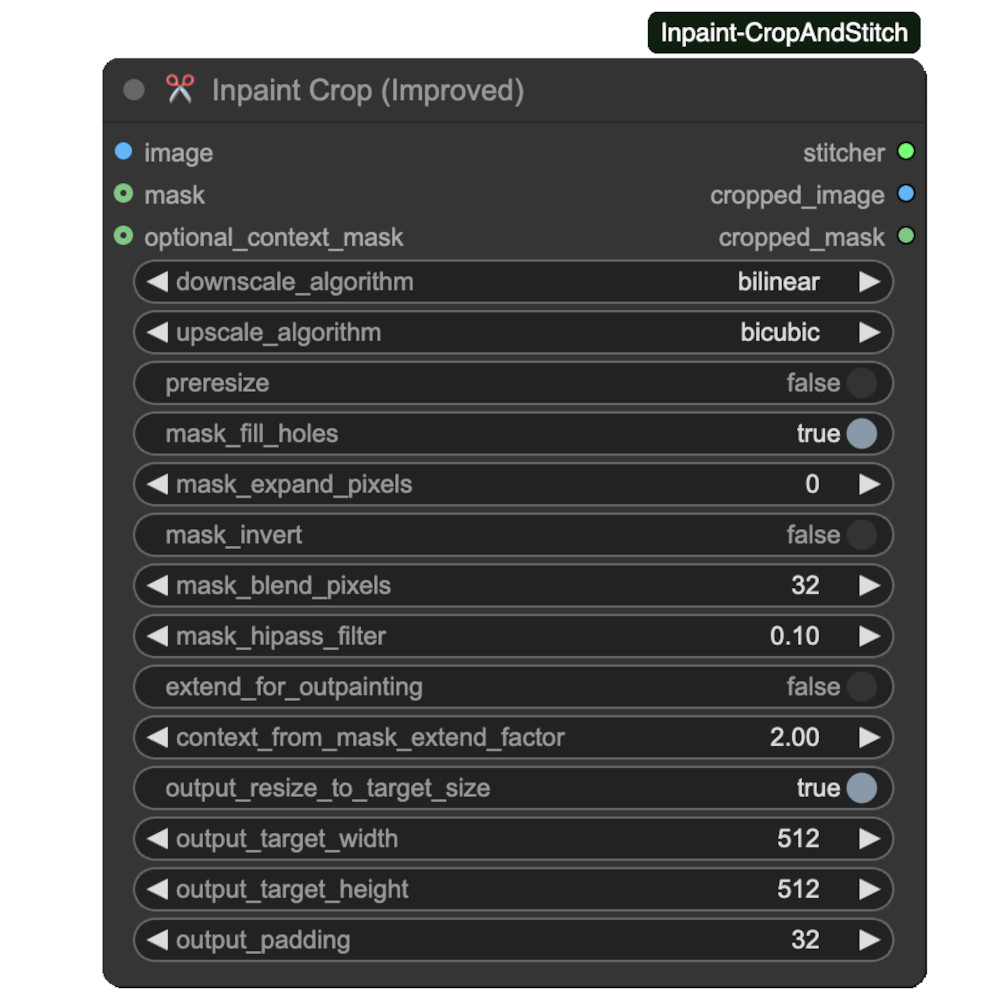
\includegraphics[width=\linewidth,height=\linewidth,valign=t]{iconinpaint.jpg} &
\textbf{Inpaint Crop and Stitch} ComfyUI nodes \SmallEntryGap
Developed ComfyUI nodes for generative artificial intelligence image inpainting that increase prompt adherence, output quality, and performance by cropping the image around the masked area, resizing it to the model's preferred resolution, and then seamlessly restitching and blending it back in place. \SmallEntryGap
Achieved \textbf{700K downloads} and \textbf{1.1K GitHub stars}. \SmallEntryGap
Links: \href{https://registry.comfy.org/nodes/comfyui-inpaint-cropandstitch}{Comfy Registry}, \href{https://github.com/lquesada/ComfyUI-Inpaint-CropAndStitch}{GitHub} \\ \portfoliospacing \\


\includegraphics[width=\linewidth,height=\linewidth,valign=t]{iconqft8.jpg} &
\textbf{qFT8} Android Application for Amateur Radio \SmallEntryGap
Developed an Android application for amateur radio communication using the FT8 digital mode with a portable transceiver. This application became the gold standard for portable FT8 operations. \SmallEntryGap
Achieved \textbf{600+ monthly users} and a rating of \textbf{4.6/5}. \SmallEntryGap
Links: \href{https://qft8.com/}{Homepage}, \href{https://play.google.com/store/apps/details?id=com.ft8.app}{Google Play Store}, \href{https://github.com/lquesada/qFT8}{GitHub}, \href{https://github.com/lquesada/qFT8/releases/tag/main}{Direct Download} \\ \portfoliospacing \\

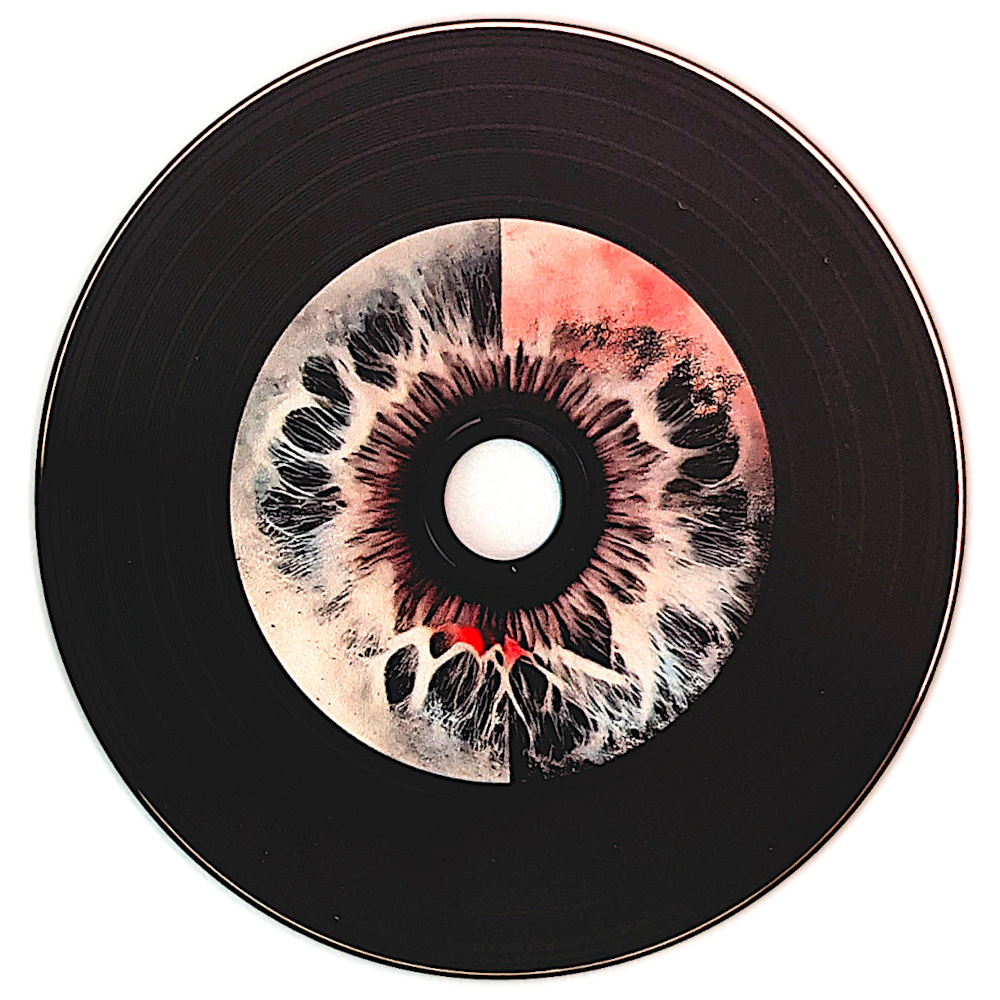
\includegraphics[width=\linewidth,height=\linewidth,valign=t]{iconwindlereye.jpg} &
\textbf{Windlereye} Music Project \SmallEntryGap
Created a fictional alternative rock band leveraging generative artificial intelligence. Wrote the lyrics to over 200 original songs, ran a manual iterative process to generate them, and did heavy post-production to ensure high audio quality. \SmallEntryGap
Achieved \textbf{50K streams}. \newline
Presented as a keynote in the \textit{GenAI Zürich 2026} conference. \SmallEntryGap
Links: \href{https://www.windlereye.com}{Homepage}, \href{https://open.spotify.com/artist/6GdiI8ZKeWhSY73WWOhbep}{Spotify}, \href{https://music.youtube.com/channel/UC4U16eJm9iTOS3j4q8_6w3w}{YouTube Music}, \href{https://www.youtube.com/@windlereye}{YouTube}, \href{https://music.apple.com/bm/artist/windlereye/1645538842}{Apple Music}, \href{https://wall.cdclick-europe.com/projects/windlereye-there-is-only-so-much-time}{Shop}, \href{https://github.com/elezetamusic/elezetamusic.github.io}{Direct Download} \\ \portfoliospacing \\

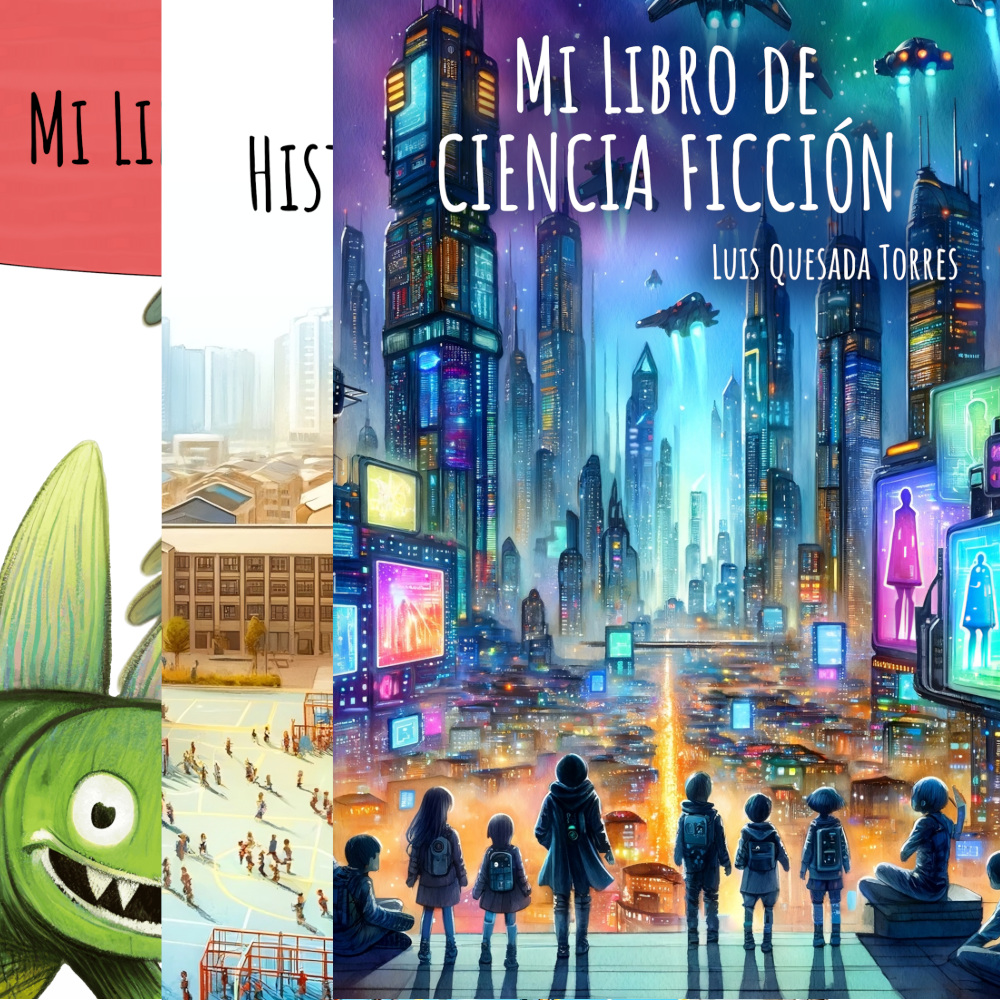
\includegraphics[width=\linewidth,height=\linewidth,valign=t]{iconbooks.jpg} &
\textbf{Mi Libro De} Book Series \SmallEntryGap
Leveraged generative AI to author and illustrate three Spanish-language children's books. These range from interactive monster readings to humorous school adventures and science fiction tales designed to improve comprehension. \SmallEntryGap
Achieved \textbf{20K downloads} and a rating of \textbf{4.2/5} over \textbf{1000+ reviews}. \SmallEntryGap
Links: \href{https://milibrode.com/}{Homepage}, \href{https://www.amazon.es/dp/B0C4DVR9N5?binding=kindle_edition&qid=1778620270&sr=8-1&ref=dbs_dp_rwt_sb_pc_tkin}{Amazon Kindle}, \href{https://www.amazon.es/dp/B0C4DVR9N5?binding=paperback&ref_=saga_sdp_cft_dsk&qid=1778620270&sr=8-1}{Amazon Paperback}, \href{https://play.google.com/store/books/series?id=dqkvGwAAABBYsM}{Google Play Books}, \href{https://github.com/orgs/milibrode/repositories}{Direct Download} \\

\end{portfoliobody}

\end{document}
